\documentclass[12pt,a4paper]{ctexart}

\usepackage{geometry}
\usepackage{setspace}
\usepackage{amsmath,amssymb,bm}
\usepackage{booktabs}
\usepackage{graphicx}
\usepackage{float}
\usepackage{caption}
\usepackage{subcaption}
\usepackage{array}
\usepackage{enumitem}
\usepackage[numbers,sort&compress]{natbib}
\usepackage{xurl}
\usepackage[hidelinks]{hyperref}

\geometry{left=2.8cm,right=2.6cm,top=2.8cm,bottom=2.8cm}
\setstretch{1.5}
\emergencystretch=3em
\graphicspath{{figures/}}
\setlist{nosep}

\newcommand{\E}{\mathbb{E}}
\newcommand{\Var}{\operatorname{Var}}
\newcommand{\RSI}{\operatorname{RSI}}

\title{\bfseries 基于资源满意度的门诊服务能力控制模型与经验标定研究}
\author{作者：\underline{\hspace{3cm}} \quad 指导教师：\underline{\hspace{3cm}}}
\date{2026年5月}

\begin{document}

\maketitle

\begin{abstract}
大型医院门诊系统长期面临患者集中到达、服务时间随机、诊室能力不同以及医生赶工可能带来质量风险之间的多重权衡。传统门诊预约与排队模型多以平均等待时间、医生空闲时间或期望成本为优化目标，能够刻画常态运行效率，但对高峰拥堵的尾部风险和服务节奏压缩的管理边界关注不足。本文借鉴资源满意度（Resource Satisficing）与风险指数思想，构建一个用于门诊服务能力控制的模型原型。模型将单位时段可释放的标准服务工作量作为决策变量，并把超过舒适服务能力后的赶工代价表示为具有明确量纲的等价工作量惩罚，从而在同一压力指标中同时记录候诊积压、随机服务需求、能力释放和服务节奏压缩成本。本文依次建立固定服务时长下的单诊室基线模型、随机服务时长下的单诊室压力控制模型，并给出多诊室可行分流的扩展形式。考虑到数据不能直接观测诊疗质量结果，本文中的赶工惩罚解释为服务质量风险的运营代理，而非对临床质量损失的直接估计。

在求解表达上，本文采用受资源满意度启发的指数型压力风险约束刻画广义系统压力的尾部敏感性；在经验实施时，则基于到达人数均值、过度离散程度以及服务时长均值和方差进行正态近似，得到可计算的确定性压力约束。实证部分使用医院门诊2023年2月1日至2月14日和2023年8月1日至8月14日两个样本窗口的就诊、预约和医生数据完成描述性分析和参数标定。结果显示，8月样本日均挂号量为6824.86人，高于2月样本的4163.93人；两期样本平均有效问诊时长均约为4.6分钟，但挂号至开始就诊平均等待从67.70分钟上升到94.10分钟。半小时到达离散系数均明显大于1，说明泊松到达只能作为基线近似，经验模型需要显式纳入过度离散修正；服务时长呈右偏分布，医生间平均服务时长变异系数约为0.55，支持模型中对服务随机性和诊室异质性的刻画。进一步地，本文在医生-日期-半小时状态层面进行模型原型标定，用样本内安全阈值和服务用时边界生成模型目标服务用时，并比较线性型、指数型和幂函数型反馈规则对该模型目标的近似能力。结果表明三类规则均呈现负向队列响应，其中线性型在样本内原始分钟尺度上的$R^2$、RMSE和AIC表现相对较好，但拟合对象是模型生成的目标用时，不构成对真实问诊行为或在线干预效果的因果检验。

\textbf{关键词：} 门诊调度；资源满意度；排队风险；服务用时反馈；可行分流；医疗运营管理
\end{abstract}

\newpage
\begin{center}
\textbf{\Large Outpatient Service Capacity Control and Empirical Calibration Based on Resource Satisficing}
\end{center}

\noindent\textbf{Abstract:}
Outpatient departments in large hospitals must balance concentrated patient arrivals, random consultation times, heterogeneous clinic capacity, and the operational risk induced by excessive service acceleration. Classical appointment scheduling and queueing models usually optimize average waiting time, physician idle time, or expected cost. These criteria are useful for normal operating efficiency but are less sensitive to tail congestion and rarely state the operational boundary of rushed consultations. Inspired by resource satisficing and riskiness-index-based healthcare resource planning, this thesis develops a prototype model for outpatient service capacity control. The decision variable is defined as standard service workload released per time slot, and the rushing penalty is interpreted as an equivalent-workload proxy for potential quality risk rather than a direct clinical-quality estimate. A progressive model family is proposed: a single-clinic baseline model with fixed service times, a single-clinic stochastic-service model, and a multi-clinic extension with routing feasibility constraints. To improve implementability, a dimensional mapping from workload capacity to target average service time per patient is introduced, and queue-state feedback rules are then constructed as simplified policy approximations.

\noindent Empirically, two outpatient data windows, February 1--14 and August 1--14, 2023, are used for descriptive analysis and parameter calibration. The results show strong over-dispersion in half-hour arrivals, right-skewed service durations, and substantial cross-physician heterogeneity. The calibrated prototype generates model-implied target service times for doctor-date-half-hour states under sample-specific safety thresholds. Linear, exponential, and power-law feedback policies are then fitted to these model-implied targets. All three policies imply shorter target service time under higher local queue pressure, while the linear specification performs better in terms of in-sample original-scale $R^2$, RMSE, and AIC. These estimates should be interpreted as policy approximation results, not as causal evidence that shortening consultations improves outpatient performance.

\noindent\textbf{Keywords:} outpatient scheduling; resource satisficing; queueing risk; service-time feedback; feasible routing; healthcare operations

\newpage
\tableofcontents
\newpage

\section{绪论}

\subsection{研究背景与意义}

门诊预约与诊疗过程是医院服务可及性和资源利用效率的重要运营环节，其运行绩效直接影响患者等待体验、医生工作负荷和诊室服务能力。门诊通常以半日或数小时诊次为基本组织单元，并将医生可用时间划分为若干预约时段；因此，患者到达、服务时长、爽约、临时到诊、医生可用性等短周期波动，会直接传导为候诊积压、医生空闲或加班\citep{FetterThompson1966,KuiperDeMastMandjes2021,LaanVanDeVrugtOlsmanBoucherie2018}。同时，患者类别、检查依赖、辅助任务和服务时间差异会进一步放大门诊流程的不确定性\citep{SalzaruloBretthauerCoteSchultz2011,ChandMoskowitzNorrisShadeWillis2009}。已有门诊预约调度研究表明，预约规则的核心在于同步随机需求与有限服务能力，并在患者等待、医生空闲、资源利用和服务质量之间形成权衡\citep{Bailey1952,CayirliVeral2003,GuptaDenton2008,AhmadiJavid2017}。

然而，门诊服务能力的调节不能仅由服务速度的调整来完成。医疗运营研究表明，服务人员会在系统负荷上升时主动压缩服务时间或改变工作方式，但持续高负荷可能削弱服务效率，并伴随质量风险上升\citep{KcTerwiesch2009}。在门诊场景中，医生工作负荷不仅影响问诊节奏，也可能改变检查开具、诊疗沟通和后续处置等临床行为\citep{ErgunSahinGunesKocabiyikogluKeskin2022}。同时，时间压力与医生压力、职业倦怠和离职意愿相关\citep{PrasadPoplauBrownEtAl2020}，医生倦怠又与患者安全事件、低专业性行为和较低患者满意度存在显著关联\citep{PanagiotiGeraghtyJohnsonEtAl2018}。因此，门诊调度模型若将服务能力视为可无成本提高的外生变量，容易低估医生赶工对诊疗质量和服务可持续性的影响。本文据此将超过舒适服务能力后的赶工风险代理纳入广义系统压力，以刻画排队削减与服务节奏边界之间的内在权衡。

进一步地，医疗资源配置中的风险并不能由平均利用率或平均等待时间充分刻画。床位容量研究已经表明，平均占用率相同的系统可能具有截然不同的床位不可得风险和延误风险；若以服务质量为目标，容量规划应关注患者能否及时获得适当资源，而不应仅依赖平均占用率目标\citep{Green2002,BagustPlacePosnett1999}。近期医疗运营研究进一步发展出床位短缺指数和资源满意度模型，用以刻画资源短缺的概率、强度及尾部风险，并在多资源、多时段环境中实现风险均衡\citep{XieLokeSimLam2023,ZhouSimLam2022}。这些研究启示本文：门诊高峰拥堵同样具有低频高损失特征，单纯优化期望等待或期望成本不足以反映极端积压的管理后果。基于此，本文借鉴风险指数与资源满意度思想，将候诊工作量、随机服务需求、能力释放和赶工惩罚统一为广义系统压力，并采用尾部敏感的风险约束描述门诊动态调度问题。

\subsection{研究问题}

现有文献已经广泛讨论了实时拥堵、服务能力调节和服务质量风险等问题，但定量刻画候诊压力、服务节奏压缩边界和资源满意度型风险控制的门诊服务能力框架仍有待完善。受限于本文数据不能直接观测患者安全事件、诊疗准确性、投诉或满意度等临床质量结果，本文不直接估计“赶工导致的真实质量损失”，而是将其作为运营层面的等价工作量惩罚进行建模。基于这一边界，本文回答以下问题：

\begin{enumerate}
  \item 如何在统一工作量尺度下定义门诊广义系统压力，使其同时包含候诊积压、随机服务需求、服务能力释放和赶工风险代理？
  \item 如何将医生短期加速服务的潜在质量风险参数化为具有明确量纲的凸惩罚，并据此刻画排队削峰与服务节奏边界之间的权衡？
  \item 如何借鉴资源满意度思想构建尾部风险敏感的服务能力控制模型，并在固定服务时长、随机服务时长和多诊室可行分流场景下保持模型结构的一致性？
  \item 当真实到达过程存在过度离散、服务时长右偏且质量结果不可观测时，如何进行审慎的参数标定，并明确模型原型与真实在线干预之间的证据边界？
  \item 如何在服务工作量决策与平均单人服务用时之间建立量纲一致的转换关系，并比较线性型、指数型与幂函数型反馈策略对模型生成目标服务用时的样本内近似能力？
\end{enumerate}

\subsection{研究内容与方法}

为探讨上述问题，本文的主要研究内容包括：首先，界定门诊服务能力控制中的广义系统压力，将候诊积压、随机服务需求、服务能力释放和医生赶工风险代理纳入统一工作量口径；其次，构建从固定服务时长单诊室模型、随机服务时长单诊室模型到多诊室可行分流模型的递进式框架；再次，引入资源满意度启发的尾部风险约束，并在均值、方差和过度离散修正下推导可计算的确定性形式；最后，建立服务工作量决策与平均单人服务用时之间的转换关系，提出线性型、指数型和幂函数型队列反馈策略，并基于真实门诊数据完成描述性分析、参数标定和样本内策略近似比较。

本研究采用文献分析、数学建模和经验估计相结合的方法。文献分析用于梳理门诊预约调度、医疗资源风险度量和资源满意度模型的理论基础；数学建模用于刻画随机到达、随机服务时长、诊室异质性和赶工风险代理之间的关系，并在正态近似下推导指数型风险约束的确定性表达；经验估计则使用医院门诊2023年2月和2023年8月两个样本窗口的就诊、预约和医生数据完成参数标定，并以$R^2$、RMSE和AIC比较不同反馈策略对模型生成目标服务用时的样本内拟合表现。本文不声称该实证部分已经验证了真实在线调度效果；在线效果仍需通过滚动仿真或现场试点评估。

\subsection{研究创新点}

在既有门诊预约调度、医疗资源风险度量和医生工作负荷研究基础上，本文的边际贡献主要体现在三个方面。第一，将门诊运行压力从患者等待或医生空闲等单一绩效指标拓展为包含候诊工作量、随机服务需求、服务能力释放和赶工风险代理的广义系统压力，并以此作为服务能力控制的核心对象。第二，在服务工作量口径下引入具有明确量纲的凸惩罚，使排队削峰与服务节奏边界能够在同一模型中比较，但本文明确不把该惩罚解释为已被数据验证的临床质量损失。第三，将资源满意度思想从住院床位等物理资源过载风险扩展到门诊服务能力控制场景，构造尾部敏感的压力风险约束，并给出从服务工作量到平均单人服务用时的转换关系。基于真实门诊数据，本文进一步展示如何用经验阈值生成模型目标服务用时，并比较三类队列反馈策略对该目标的样本内近似能力，从而为后续滚动仿真和现场试点提供可复现的模型原型。

\section{文献综述}

\subsection{门诊预约与动态调度研究}

门诊预约调度研究长期围绕患者等待、医生空闲和加班之间的权衡展开。Bailey较早使用排队思想分析门诊预约系统\citep{Bailey1952}，Fetter和Thompson进一步指出预约间隔、服务时间、患者到达模式、爽约、临时到诊、医生到达和服务中断都会影响患者等待与医生空闲的关系\citep{FetterThompson1966}。Cayirli和Veral、Gupta和Denton以及Ahmadi-Javid等的综述表明，门诊预约研究已经形成包括排队模型、仿真、随机规划、启发式算法和动态决策在内的方法体系，研究对象也从单诊室静态预约扩展到多医生、患者偏好、爽约、实时偏差处理和多层级容量规划\citep{CayirliVeral2003,GuptaDenton2008,AhmadiJavid2017,Hulshof2012}。在具体模型上，Denton和Gupta将预约时间设计表述为随机规划问题\citep{DentonGupta2003}，Robinson和Chen提出了随机服务时间条件下的启发式规则\citep{RobinsonChen2003}；近年研究则进一步处理同日请求、移动预约窗口、动态预约和分布鲁棒调度等问题\citep{BalasubramanianBiehlDaiMuriel2014,DaiGengXie2021,LaanVanDeVrugtOlsmanBoucherie2018,ZhangShenErdogan2017}。这些研究为门诊调度建模提供了充分基础，但其决策重点通常在预约时点、预约容量、患者接纳或分配规则上，医生短期服务能力调节及其质量代价仍有进一步建模空间。

\subsection{医生工作负荷与服务质量研究}

门诊服务能力并非单纯的物理容量，还与医生工作节奏和服务质量有关。医疗运营研究发现，系统负荷上升会影响服务时间和患者安全，说明服务速度调整可能伴随质量风险\citep{KcTerwiesch2009}。在门诊或相近诊疗场景中，医生未完成工作量会改变检查开具行为，时间压力会影响医生压力、职业倦怠和离职意愿，医生倦怠也与患者安全事件、低专业性行为和较低患者满意度相关\citep{ErgunSahinGunesKocabiyikogluKeskin2022,PrasadPoplauBrownEtAl2020,PanagiotiGeraghtyJohnsonEtAl2018}。因此，在门诊服务能力控制中，服务能力提升应同时考虑排队削减收益和服务节奏压缩风险。本文将医生超过舒适服务能力后的代价表示为凸惩罚，并将其作为运营代理纳入广义系统压力。

\subsection{相关理论模型与分析方法}

门诊调度研究常用的理论模型主要包括排队模型、随机规划、动态规划、仿真优化和鲁棒优化。排队模型适合刻画患者到达、服务时间和候诊积压之间的基本关系；随机规划和仿真优化能够处理服务时长、爽约和临时到诊等随机因素；动态规划和马尔可夫决策过程适用于预约请求逐步到达、系统状态随时间更新的调度问题\citep{DentonGupta2003,RobinsonChen2003,BalasubramanianBiehlDaiMuriel2014,DaiGengXie2021}。在分布信息不完全的情况下，分布鲁棒优化进一步通过矩信息或支撑集构造模糊集，用于处理随机服务时长和爽约行为的不确定性\citep{ZhangShenErdogan2017}。

在医疗资源风险分析中，Aumann和Serrano提出的风险指数从分布整体出发度量风险，为后续医疗资源短缺指数提供了理论基础\citep{AumannSerrano2008,XieLokeSimLam2023}。Zhou、Sim和Lam的资源满意度模型将该类思想用于多资源、多时段住院提前排班，强调在不确定需求下控制资源过载尾部风险\citep{ZhouSimLam2022}。本文借鉴上述方法，将门诊时段压力写成包含均值、方差和安全裕度的风险约束，并通过正态近似得到可计算的确定性表达。

\subsection{文献述评与研究定位}

综上，既有研究已经较系统地讨论了门诊预约时间设计、随机服务时长、爽约、动态接纳、多医生调度以及风险规避型预约优化，为本文提供了成熟的建模基础。与此同时，医生工作负荷文献表明高负荷会影响服务时间、诊疗行为和服务质量，医疗资源风险文献则说明平均利用率和平均等待不足以刻画资源短缺的尾部风险。上述两类发现与门诊调度问题密切相关，但在现有门诊优化模型中通常没有被统一为一个可直接用于服务能力控制的压力指标。

基于此，本文将研究定位于门诊服务能力控制：一方面，将候诊工作量、随机服务需求、服务能力释放和医生赶工风险代理统一为广义系统压力；另一方面，将资源满意度启发的尾部风险约束引入门诊场景，并通过队列反馈型平均服务用时函数把模型目标转化为现场可理解的服务节奏提示。该定位既延续门诊预约调度研究对等待、空闲和加班权衡的关注，也吸收医疗资源风险度量对尾部过载的处理思想，从而为高峰拥堵下的门诊服务能力调节提供更贴近实际运行的分析框架。

\section{问题描述与模型假设}

\subsection{门诊系统与队列状态}

本文考虑一个离散时间门诊系统。一天被划分为$T$个长度为$\Delta$的决策时段，实证部分取$\Delta=30$分钟。时段$t$开始时，系统已知当前候诊工作量$W_t$，单位为分钟，表示若不再有新患者到达，消化现有队列所需的服务时间。

时段$t$的决策变量为$c_t$，表示该时段释放的服务工作量，单位为分钟。服务完成后的实际队列状态满足
\begin{equation}
\tilde W_{t+1}=\left[W_t+\tilde D_t-c_t\right]_+,
\end{equation}
其中$\tilde D_t$为时段$t$新到患者形成的随机服务需求，$[x]_+=\max\{x,0\}$。在优化模型中，本文使用条件均值更新预测状态，即$W_{t+1}=[W_t+\E(\tilde D_t)-c_t]_+$；在现场更新时，每个时段开始后再用实际观测到的队列状态修正下一时段决策。

\subsection{随机到达与随机服务需求}

令$\tilde A_t$表示时段$t$的到达人数。为避免把泊松到达作为不可检验前提，本文采用均值--方差口径描述短时段到达过程：
\begin{equation}
\E(\tilde A_t)=\lambda_t,\qquad \Var(\tilde A_t)=\kappa_t\lambda_t,\qquad \kappa_t>0,
\end{equation}
其中$\lambda_t$为该时段平均到达率，$\kappa_t$为到达离散系数。$\kappa_t=1$时退化为泊松到达；$\kappa_t>1$表示短时段到达存在过度离散和峰值聚集。设第$k$名患者的服务需求为$S_k$，满足独立同分布且具有有限均值和方差：
\begin{equation}
S_k\overset{i.i.d.}{\sim}F_S,\qquad m=\E(S_k),\quad v=\Var(S_k)<\infty .
\end{equation}
则时段总服务需求为随机和
\begin{equation}
\tilde D_t=\sum_{k=1}^{\tilde A_t}S_k,
\end{equation}
并有
\begin{equation}
\E(\tilde D_t)=\lambda_t m,\qquad
\Var(\tilde D_t)=\lambda_t v+\kappa_t\lambda_t m^2
=\lambda_t(v+\kappa_t m^2).
\label{eq:compound-moments}
\end{equation}
在需要使用指数矩的理论表达中，还需假定服务需求在相关参数邻域内具有有限矩母函数，或在运营实施中采用截尾后的经验分布。本文实证部分剔除超过60分钟的异常问诊时长，并主要使用均值、方差和离散系数进行正态近似，因此所得结果应理解为可计算的风险近似，而非对原始重尾分布的精确解析解。

\subsection{服务能力调节与赶工风险代理}

门诊高峰期可以通过提高服务节奏释放更多能力，但该调节存在质量边界。本文用凸函数刻画超过舒适服务能力后的赶工风险代理：
\begin{equation}
h(c_t)=\gamma[c_t-c_0]_+^2,\qquad \gamma>0,
\label{eq:rushing-penalty}
\end{equation}
其中$c_0$为舒适服务能力基准，$\gamma$为赶工惩罚系数。由于$c_t$以分钟工作量计量，$\gamma$的单位为“每分钟”，从而$h(c_t)$仍可解释为等价工作量分钟。该惩罚不是直接观测到的医疗质量损失，而是把持续压缩服务节奏可能造成的沟通不足、诊疗遗漏和医生疲劳风险转换为运营层面的安全裕度消耗。固定服务时长模型是上一小节随机服务需求形式的特殊情形，即$m=s_{\mathrm{base}}$且$v=0$。

\subsection{模型假设与递进结构}

为保持模型清晰，本文作如下假设。第一，短期预测窗口内的到达均值$\lambda_t$和离散系数$\kappa_t$可由历史到达、预约信息和实时到院情况估计。第二，服务需求与到达过程在给定时段内相互独立，且服务需求至少具有有限二阶矩；若使用原始指数风险约束，则进一步要求矩母函数在局部存在。第三，服务能力存在上下界$c_{\min}\leq c_t\leq c_{\max}$，以反映医生工作节奏的可调范围，且$c_{\max}$只能解释为短时应急边界。第四，本文研究对象为门诊运行层面的服务能力控制，不直接处理诊断决策、个体患者临床优先级和真实跨科室转诊规则。

在此基础上，本文构建三类模型。Model 1假设服务时长固定，用于给出单诊室服务能力控制的基线；Model 2引入随机服务时长和到达过度离散修正，用于刻画服务需求方差对尾部风险的影响；Model 3进一步考虑多诊室可行分流和诊室异质性。由于本文数据不包含真实在线重分流记录，Model 3在实证中作为扩展框架而非已验证的现场分流算法。

\begin{figure}[H]
  \centering
  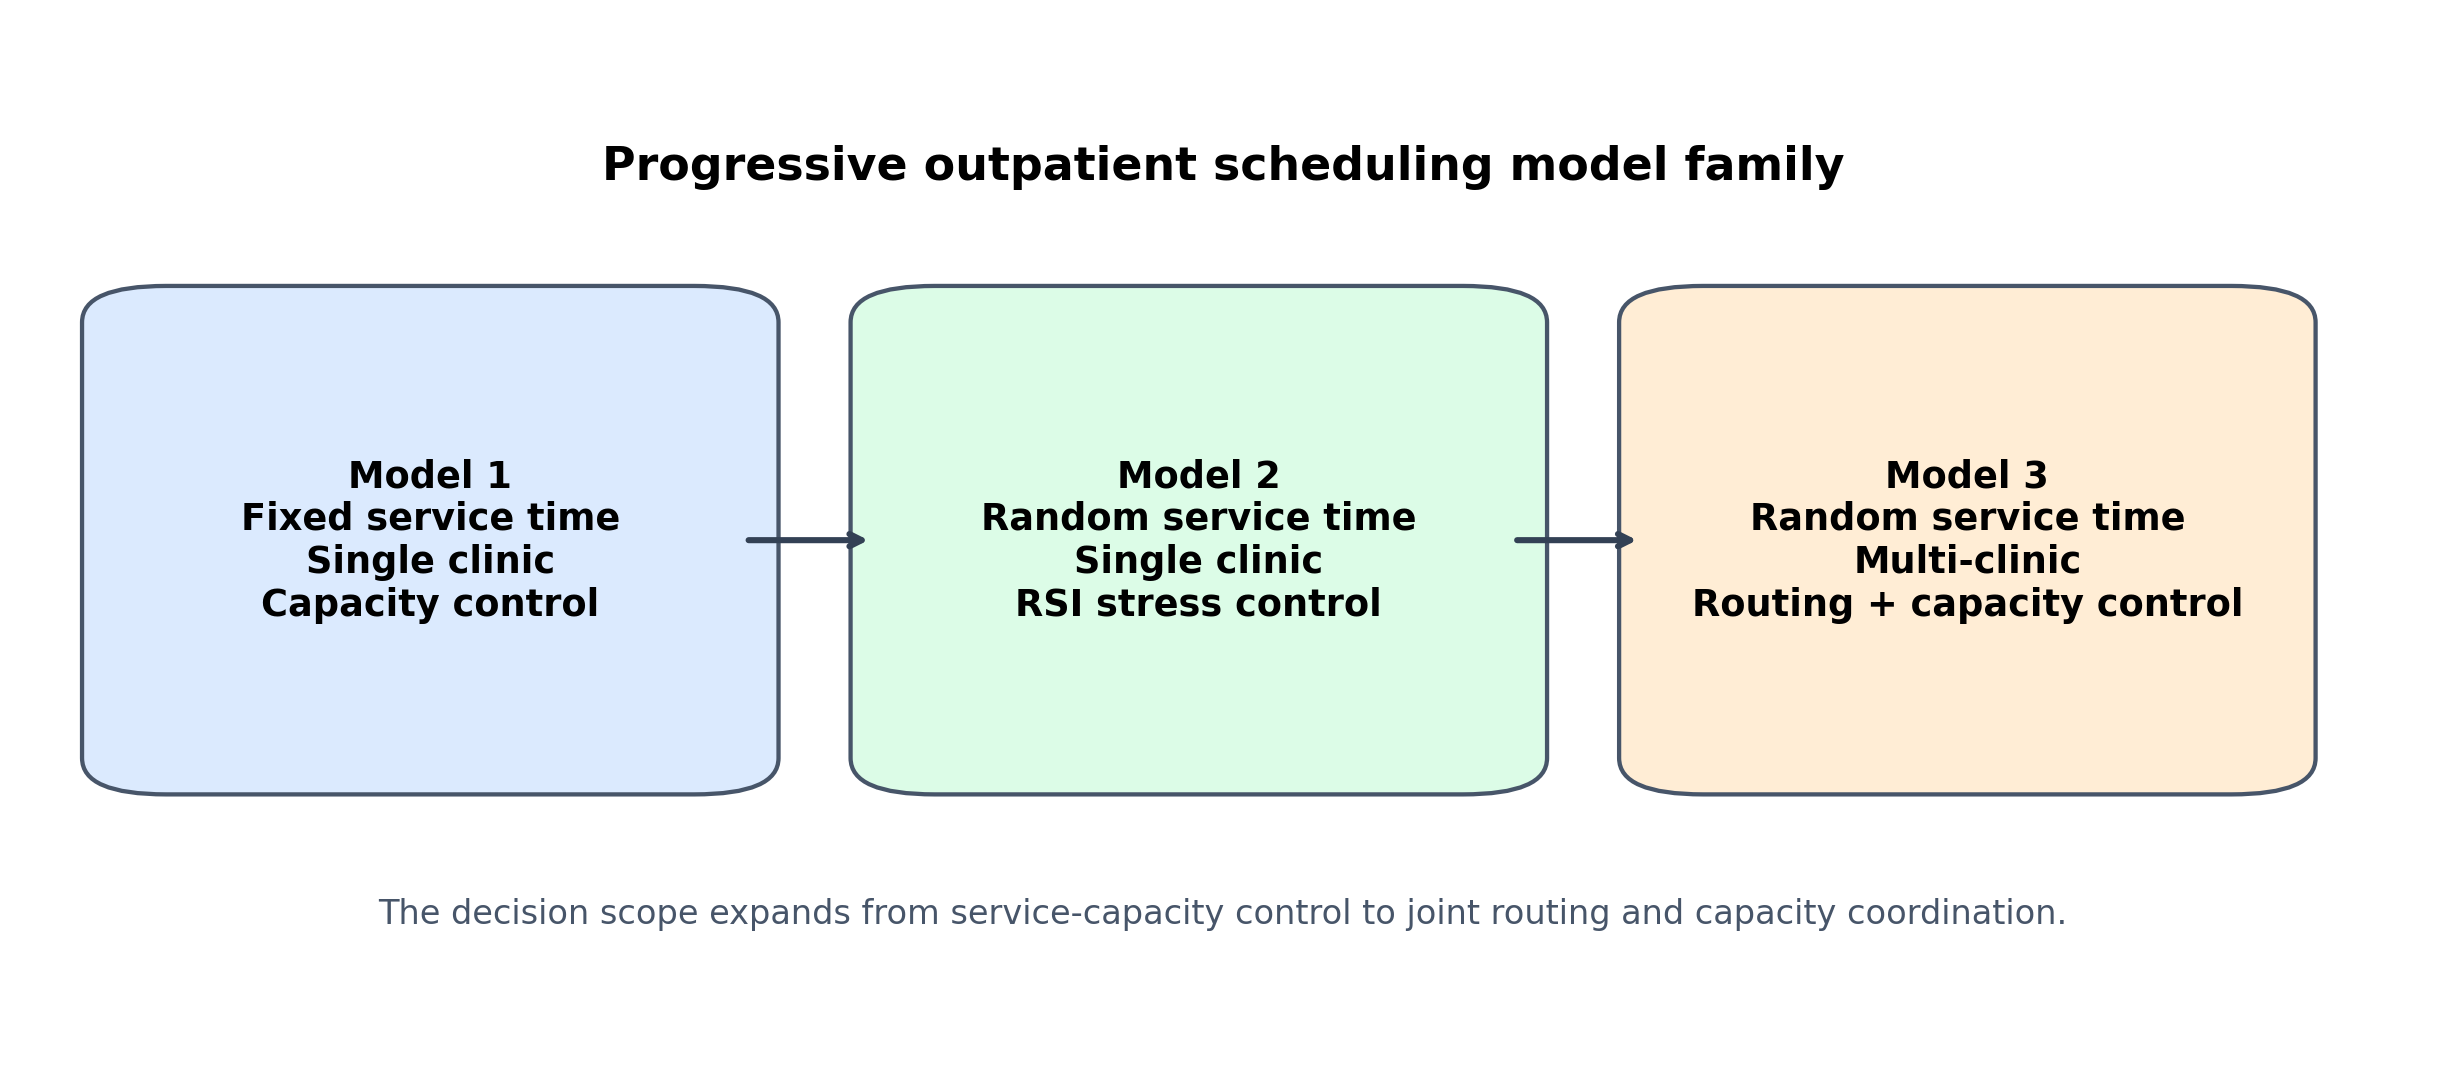
\includegraphics[width=0.92\textwidth]{model_framework.png}
  \caption{门诊服务能力控制模型体系}
  \label{fig:model-framework}
\end{figure}

\section{基于广义系统压力的服务能力控制模型}

\subsection{广义系统压力定义}

给定时段开始状态$W_t$和服务能力决策$c_t$，本文定义时段$t$的广义系统压力为
\begin{equation}
L_t=W_t+\tilde D_t-c_t+h(c_t).
\label{eq:general-pressure}
\end{equation}
其中$W_t+\tilde D_t-c_t$刻画服务能力释放后的剩余工作量，$h(c_t)$刻画过度加速带来的等价工作量惩罚。该指标能够反映候诊积压和随机服务需求会提高压力，服务能力释放会降低压力，赶工风险代理会在服务能力过高时重新增加压力。

\subsection{资源满意度启发的尾部风险约束}

借鉴风险指数和资源满意度思想\citep{AumannSerrano2008,ZhouSimLam2022,XieLokeSimLam2023}，本文采用指数型压力风险约束：
\begin{equation}
\E\left[\exp\left(\frac{L_t-C_{\mathrm{safe}}}{\rho\nu}\right)\right]\leq 1,
\label{eq:rsi-constraint}
\end{equation}
其中$C_{\mathrm{safe}}$为压力安全阈值，$\nu>0$为风险敏感度参数，$\rho>0$为待最小化的风险水平。式\eqref{eq:rsi-constraint}通过指数函数放大$L_t$右尾，当压力均值接近阈值或波动变大时，满足约束所需的$\rho$随之升高。该表达的精确使用要求$L_t$的指数矩存在；在本文经验部分，风险约束通过正态近似转化为均值--方差形式，因此只作为尾部敏感的可计算近似。资源满意度启发的压力风险指数定义为
\begin{equation}
\RSI_{\nu}(L_t,C_{\mathrm{safe}})
=\inf\left\{\rho>0:
\E\left[\exp\left(\frac{L_t-C_{\mathrm{safe}}}{\rho\nu}\right)\right]\leq 1
\right\}.
\end{equation}
理论模型在调度周期内最小化所有时段的最大风险水平，即在满足服务能力上下界和队列状态更新约束的条件下，使最不利时段的广义压力风险尽可能低。后文实证不直接求解完整动态优化问题，而是在医生局部状态上使用该约束生成目标服务工作量，用于检验模型原型是否能给出可解释的服务用时建议。

\subsection{Model 1：固定服务时长下的单诊室服务能力控制}

固定服务时长模型用于建立基础标准。设每名患者服务需求为$s_{\mathrm{base}}$，则$\tilde D_t=s_{\mathrm{base}}\tilde A_t$，$\E(\tilde D_t)=\lambda_ts_{\mathrm{base}}$，$\Var(\tilde D_t)=\kappa_t\lambda_ts_{\mathrm{base}}^2$，广义压力为
\begin{equation}
L_t^{(1)} = W_t+\tilde A_t s_{\mathrm{base}}-c_t+\gamma[c_t-c_0]_+^2.
\label{eq:model1-pressure}
\end{equation}
对应的服务能力控制模型为
\begin{equation}
\begin{aligned}
\min_{\bm{c},\rho}\quad & \rho\\
\mathrm{s.t.}\quad
& \E\left[\exp\left(\frac{L_t^{(1)}-C_{\mathrm{safe}}}{\rho\nu}\right)\right]\leq 1,\quad t=1,\ldots,T,\\
& W_{t+1}=\max\{0,W_t+\lambda_t s_{\mathrm{base}}-c_t\},\\
& c_{\min}\leq c_t\leq c_{\max},\quad t=1,\ldots,T.
\end{aligned}
\label{eq:model1}
\end{equation}
该模型仅保留到达随机性，适用于服务时长波动较小或希望建立基线比较的场景。若实证显示$\kappa_t>1$，则不能把该模型解释为严格泊松排队系统，而应将其视为含过度离散修正的固定服务需求近似。

\subsection{Model 2：随机服务时长下的单诊室压力控制}

随机服务时长模型是本文的核心单诊室模型。根据式\eqref{eq:compound-moments}，总服务需求$\tilde D_t$同时受患者到达人数和患者服务时长影响。广义压力为
\begin{equation}
L_t^{(2)}=W_t+\tilde D_t-c_t+\gamma[c_t-c_0]_+^2.
\label{eq:model2-pressure}
\end{equation}
优化模型为
\begin{equation}
\begin{aligned}
\min_{\bm{c},\rho}\quad & \rho\\
\mathrm{s.t.}\quad
& \E\left[\exp\left(\frac{L_t^{(2)}-C_{\mathrm{safe}}}{\rho\nu}\right)\right]\leq 1,\quad t=1,\ldots,T,\\
& W_{t+1}=\max\{0,W_t+\lambda_t m-c_t\},\\
& c_{\min}\leq c_t\leq c_{\max},\quad t=1,\ldots,T.
\end{aligned}
\label{eq:model2}
\end{equation}
与Model 1相比，Model 2将服务时长方差纳入风险约束。即使平均服务时长相同，服务时长波动越大，广义压力右尾越厚，模型所需的安全裕度也越高。

\subsection{Model 3：多诊室可行分流与协同服务能力控制}

大型门诊通常由多个诊室共同服务。设诊室集合为$I=\{1,\ldots,n\}$，时段$t$分配给诊室$i$的患者比例为$p_{it}$。现实中患者只能被分配到具有相应科室、号源和医生资质的诊室，故令$e_{it}\in\{0,1\}$表示诊室$i$在时段$t$是否可接收该类需求，并要求
\begin{equation}
\sum_{i\in I}p_{it}=1,\qquad 0\leq p_{it}\leq e_{it}.
\end{equation}
为保证分流问题可行，需要对每个时段满足$\sum_{i\in I}e_{it}\geq1$。若按患者类别或科室分别建模，则可进一步把$p_{it}$和$e_{it}$扩展为$p_{kit}$和$e_{kit}$，其中$k$表示患者类别或科室需求。
在均值--方差口径下，诊室$i$的到达满足
\begin{equation}
\E(\tilde A_{it})=\lambda_t p_{it},\qquad
\Var(\tilde A_{it})=\kappa_{it}\lambda_t p_{it},
\end{equation}
其中$\kappa_{it}$刻画诊室局部到达的过度离散。若诊室$i$的服务需求均值和方差分别为$m_i$和$v_i$，则随机服务需求为
\begin{equation}
\tilde D_{it}=\sum_{k=1}^{\tilde A_{it}}S_{ik}.
\end{equation}
诊室$i$的广义压力为
\begin{equation}
L_{it}^{(3)}=W_{it}+\tilde D_{it}-c_{it}+\gamma_i[c_{it}-c_{i0}]_+^2.
\label{eq:model3-pressure}
\end{equation}
多诊室优化模型为
\begin{equation}
\begin{aligned}
\min_{\bm{c},\bm{p},\rho}\quad & \rho\\
\mathrm{s.t.}\quad
& \E\left[\exp\left(\frac{L_{it}^{(3)}-C_{\mathrm{safe},i}}{\rho\nu}\right)\right]\leq 1,\quad i\in I,\ t=1,\ldots,T,\\
& \sum_{i\in I}p_{it}=1,\quad 0\leq p_{it}\leq e_{it},\quad i\in I,\ t=1,\ldots,T,\\
& W_{i,t+1}=\max\{0,W_{it}+\lambda_t p_{it}m_i-c_{it}\},\\
& c_{\min,i}\leq c_{it}\leq c_{\max,i},\quad i\in I,\ t=1,\ldots,T.
\end{aligned}
\label{eq:model3}
\end{equation}
该模型同时调节分流比例和诊室服务能力。若某诊室队列压力较高或赶工惩罚较大，模型会在可行分流集合内降低其分流比例或要求其他合格诊室承担更多需求；若某诊室仍有安全裕度，则可承担更多患者。该表达没有覆盖患者已经进入特定医生队列后的重新叫号成本、患者偏好和临床优先级，因此在没有现场分流记录时不应被解释为已部署的实时分诊规则。

需要说明的是，Model 1--Model 3的作用是给出统一的压力定义、风险约束和服务能力边界。本文不展开完整跨时段优化问题的全局求解算法，也不声称后续经验部分求解了上述完整模型；第五章只使用其确定性局部风险约束生成医生-时段层面的目标服务工作量。

\section{模型转化与策略实现}

\subsection{随机和服务需求的矩与正态近似}

第4章模型的随机性主要来自随机到达人数与随机服务需求形成的随机和。令$\E(\tilde A_t)=\lambda_t$、$\Var(\tilde A_t)=\kappa_t\lambda_t$，$\tilde D_t=\sum_{k=1}^{\tilde A_t}S_k$，且$S_k$独立同分布、$\E(S_k)=m$、$\Var(S_k)=v<\infty$。由随机和的矩公式可得
\begin{equation}
\E(\tilde D_t)=\lambda_t m,\qquad
\Var(\tilde D_t)=\lambda_t(v+\kappa_t m^2).
\end{equation}
当$\lambda_t$较大、单个患者服务需求不存在极端重尾主导、到达过程可由均值和方差稳定刻画，且到达随机变量本身满足适当的渐近正态性或可由负二项等计数分布近似时，随机和中心极限定理给出如下近似\citep{Ross2014}：
\begin{equation}
\frac{\tilde D_t-\lambda_t m}{\sqrt{\lambda_t(v+\kappa_t m^2)}}
\Rightarrow N(0,1).
\label{eq:compound-clt}
\end{equation}
该结果说明，在上述条件下可用
\begin{equation}
\tilde D_t\approx N\left(\lambda_t m,\lambda_t(v+\kappa_t m^2)\right)
\end{equation}
近似总服务需求。该近似把随机服务需求压缩为均值、方差和到达离散系数三个量，为后续确定性转化提供基础。若某些时段到达量很小、到达过程具有强相关聚集，或服务需求呈明显重尾，则应使用经验分布、负二项到达或离散事件仿真检验近似误差。本文后续实证结果因此仅解释为模型原型的样本内标定。

\subsection{指数型风险约束的确定性转化}

式\eqref{eq:rsi-constraint}包含随机变量的指数矩。在上述正态近似下，设$X\sim N(\mu_X,\sigma_X^2)$，则
\begin{equation}
\E\left[\exp\left(\frac{X-C}{\rho\nu}\right)\right]
=\exp\left(\frac{\mu_X-C}{\rho\nu}+\frac{\sigma_X^2}{2\rho^2\nu^2}\right).
\end{equation}
令该值不超过1，得到
\begin{equation}
\rho \geq \frac{\sigma_X^2}{2\nu(C-\mu_X)},\qquad C>\mu_X.
\label{eq:normal-rsi}
\end{equation}
等价地，对给定$\rho$，有
\begin{equation}
\sigma_X^2+2\rho\nu\mu_X\leq 2\rho\nu C.
\label{eq:rsi-deterministic}
\end{equation}
若$C\leq\mu_X$，则该时段的平均压力已经超过安全阈值，单纯依靠方差修正无法满足约束，需要提高服务能力上限、改变分流或重新设定安全阈值。因此，后续经验标定会同时报告触及服务用时下界的状态比例，而不把这些状态解释为已经被模型完全消除的风险。

对Model 2，广义压力的均值和方差为
\begin{equation}
\E[L_t^{(2)}]=W_t+\lambda_t m-c_t+\gamma[c_t-c_0]_+^2,
\end{equation}
\begin{equation}
\Var(L_t^{(2)})=\lambda_t(v+\kappa_t m^2).
\end{equation}
将其代入式\eqref{eq:rsi-deterministic}，得到单诊室随机服务模型的确定性风险约束：
\begin{equation}
\lambda_t(v+\kappa_t m^2)
 +2\rho\nu\left\{W_t+\lambda_t m-c_t+\gamma[c_t-c_0]_+^2\right\}
\leq 2\rho\nu C_{\mathrm{safe}},
\quad t=1,\ldots,T.
\label{eq:model2-deterministic-rsi}
\end{equation}
对Model 3，诊室$i$的均值和方差为
\begin{equation}
\E[L_{it}^{(3)}]=W_{it}+\lambda_t p_{it}m_i-c_{it}+\gamma_i[c_{it}-c_{i0}]_+^2,
\end{equation}
\begin{equation}
\Var(L_{it}^{(3)})=\lambda_t p_{it}(v_i+\kappa_{it}m_i^2).
\end{equation}
对应的多诊室确定性风险约束为
\begin{equation}
\begin{aligned}
&\lambda_t p_{it}(v_i+\kappa_{it}m_i^2)
 +2\rho\nu\left\{W_{it}+\lambda_t p_{it}m_i-c_{it}
 +\gamma_i[c_{it}-c_{i0}]_+^2\right\}\\
&\qquad\leq 2\rho\nu C_{\mathrm{safe},i},
\quad i\in I,\ t=1,\ldots,T.
\end{aligned}
\label{eq:model3-deterministic-rsi}
\end{equation}
式\eqref{eq:model2-deterministic-rsi}和式\eqref{eq:model3-deterministic-rsi}显示，风险约束由三部分构成：服务需求方差、平均剩余工作量和赶工风险代理。

\subsection{从服务能力决策到服务用时反馈}

第4章模型以单位时段释放的服务工作量$c_{it}$为决策变量，便于统一刻画候诊积压、随机服务需求和赶工风险代理。接下来据此进一步推导平均每位患者的目标服务用时。

设$\Delta$为单个决策时段长度，$N_{it}$为诊室$i$在时段$t$可用的等效出诊单元数，$m_i$为该诊室在舒适节奏下的平均标准服务需求，$s_{it}$为该时段建议执行的平均单人服务用时。这里的$c_{it}$不是实际钟表时间，而是折算后的标准工作量释放量：若医生用低于舒适均值的时间完成一个平均病例，模型认为同一时段释放了更多标准工作量，但同时通过$h(c_{it})$消耗安全裕度。在时段内服务节奏近似稳定时，诊室$i$可服务的患者数约为$N_{it}\Delta/s_{it}$，对应的标准化服务工作量为
\begin{equation}
c_{it}(s_{it})=\frac{N_{it}\Delta m_i}{s_{it}}.
\label{eq:capacity-duration-map}
\end{equation}
当$s_{it}=m_i$时，式\eqref{eq:capacity-duration-map}给出$c_{it}=N_{it}\Delta$，即舒适节奏下可释放的标准工作量；当$s_{it}<m_i$时，同一时段内可释放的标准工作量上升，但赶工惩罚$h(c_{it})$也随之增加。该转换仅用于运营节奏建议，不能要求医生对所有患者机械缩短问诊时间；复杂病例、复诊解释和临床沟通仍应优先服从医疗判断。
反过来，若模型求得目标服务工作量$c_{it}^{*}$，则现场可执行的目标平均服务用时为
\begin{equation}
s_{it}^{*}=\frac{N_{it}\Delta m_i}{c_{it}^{*}},
\label{eq:duration-from-capacity}
\end{equation}
并需满足$s_{\min}\leq s_{it}^{*}\leq s_{\max}$。其中$s_{\min}$应由临床安全边界、管理规则或审慎的数据分位数共同确定。若实证只能使用数据分位数，则$s_{\min}$只能解释为原型标定边界，而非已由临床质量结果验证的最短安全问诊时间。因此，队列反馈策略并非脱离优化模型的独立经验式，而是对式\eqref{eq:duration-from-capacity}所对应模型目标服务用时的参数化近似。

设$Q_{it}$为时段开始时诊室$i$名下的待诊人数，$q_{it}=Q_{it}/N_{it}$表示平均每个出诊单元面对的局部队列长度。给定任一反馈函数$f(q_{it};\theta)$，其诱导的服务能力决策为
\begin{equation}
c_{it}(\theta)=\frac{N_{it}\Delta m_i}{f(q_{it};\theta)}.
\label{eq:feedback-capacity}
\end{equation}
将式\eqref{eq:feedback-capacity}代入广义系统压力，可得参数化策略下的压力表达：
\begin{equation}
L_{it}(\theta)=W_{it}+\tilde D_{it}
-\frac{N_{it}\Delta m_i}{f(q_{it};\theta)}
+\gamma_i\left[\frac{N_{it}\Delta m_i}{f(q_{it};\theta)}-c_{i0}\right]_+^2.
\label{eq:feedback-pressure}
\end{equation}
式\eqref{eq:feedback-pressure}说明，反馈函数通过改变平均服务用时影响服务能力释放，并进一步进入广义压力和风险约束。

本文首先定义线性型反馈函数：
\begin{equation}
s_{it}^{L}(q_{it})=\min\{s_{\max},\max[s_{\min},a_L-b_Lq_{it}]\},\qquad b_L\geq0.
\label{eq:feedback-linear}
\end{equation}
其次定义指数型反馈函数：
\begin{equation}
s_{it}^{E}(q_{it})=\min\{s_{\max},\max[s_{\min},a_E\exp(-b_Eq_{it})]\},\qquad b_E\geq0.
\label{eq:feedback-exp}
\end{equation}
进一步定义幂函数型反馈函数：
\begin{equation}
s_{it}^{P}(q_{it})=\min\{s_{\max},\max[s_{\min},a_P(1+q_{it})^{-b_P}]\},\qquad b_P\geq0.
\label{eq:feedback-power}
\end{equation}
其中$s_{it}^{L}(q_{it})$、$s_{it}^{E}(q_{it})$和$s_{it}^{P}(q_{it})$为时段$t$诊室$i$建议的平均单人服务用时，$a_L$、$a_E$和$a_P$表示低队列压力下的基础服务时长，$b_L$、$b_E$和$b_P$表示队列压力对平均服务用时的压缩强度，$s_{\min}$和$s_{\max}$分别表示临床上可接受的服务用时下界和上界。



\section{数据处理、参数标定与实证分析}

\subsection{数据来源与清洗口径}

本文使用\texttt{data.ods}中的医院门诊业务数据，包含两个样本窗口：2023年2月1日至2023年2月14日，以及2023年8月1日至2023年8月14日。每个窗口包括就诊记录、预约时段和医生信息三类表。就诊记录包含挂号时间、叫号时间、开始就诊时间、后续检查缴费取药时间、科室名称、医生ID和患者分类；预约表包含医生开诊日期、预约区间容量和预约数；医生表包含医生样本信息。两个窗口均为短期样本，能够用于展示季节性高低负荷差异和模型标定流程，但不足以支持长期季节规律或干预效果的因果判断。

清洗时，本文将开始就诊后最早出现的“就诊检查时间、首次付费时间、最后付费时间、检验时间、检查时间、发药时间、结束就诊时间”作为医生释放患者的代理结束时点，并剔除有效问诊时长超过60分钟的异常记录。该口径的优点是可以在缺少精确离室时间的情况下构造可复现的服务时长指标；局限是该指标可能混入检查、缴费或系统记录延迟，也可能产生极短服务时长。因此，本文将其称为“有效问诊时长代理”，并在解释时避免把它等同于严格的医生面对面诊疗时间。等待时间也以挂号至开始就诊为主，该指标可能包含患者提前挂号或提前到院时间；叫号至开始就诊等待仅作为辅助描述，不直接进入模型标定。

\begin{table}[H]
\centering
\small
\caption{样本窗口核心运营指标}
\label{tab:descriptive-statistics}
\begin{tabular}{lrr}
\toprule
指标 & 2023年2月样本 & 2023年8月样本 \\
\midrule
就诊记录数 & 58,295 & 95,548 \\
预约时段数 & 5,372 & 6,365 \\
医生样本数 & 366 & 427 \\
日均挂号量（人） & 4163.93 & 6824.86 \\
平均服务时长（分钟） & 4.61 & 4.62 \\
服务时长95\%分位数（分钟） & 12.97 & 11.78 \\
挂号至开始就诊平均等待（分钟） & 67.70 & 94.10 \\
挂号至开始就诊95\%分位数（分钟） & 260.69 & 334.36 \\
预约区间平均利用率 & 0.73 & 0.81 \\
满载预约区间占比 & 53.40\% & 61.62\% \\
\bottomrule
\end{tabular}
\end{table}


表\ref{tab:descriptive-statistics}显示，8月样本就诊记录数和日均挂号量高于2月样本，但两期平均服务时长代理几乎相同，均约为4.6分钟。等待时间的差异则十分明显：8月挂号至开始就诊平均等待为94.10分钟，较2月的67.70分钟增加约39.0\%。这一现象提示高负荷月份的拥堵更可能与需求侧集中到达、预约负载和诊室间不均衡有关，而不能简单归因于医生平均问诊速度变化。由于本文没有进行因果分解，后续只将该结果作为模型关注到达波动和负载不均衡的经验动机。

\subsection{到达过程与服务时间分布}

图\ref{fig:arrival-profile}展示了两期样本的平均半小时到达曲线。2月样本最高到达时段出现在09:30附近，8月样本高峰明显前移到07:30。该差异说明两个样本窗口的到达节奏不同，并提示开诊初期集中挂号可能使系统在一天开始时迅速累积队列，使后续时段即使服务能力稳定也难以完全恢复。由于样本窗口较短，本文不把这一现象外推为所有高需求季节的一般规律。

\begin{figure}[H]
  \centering
  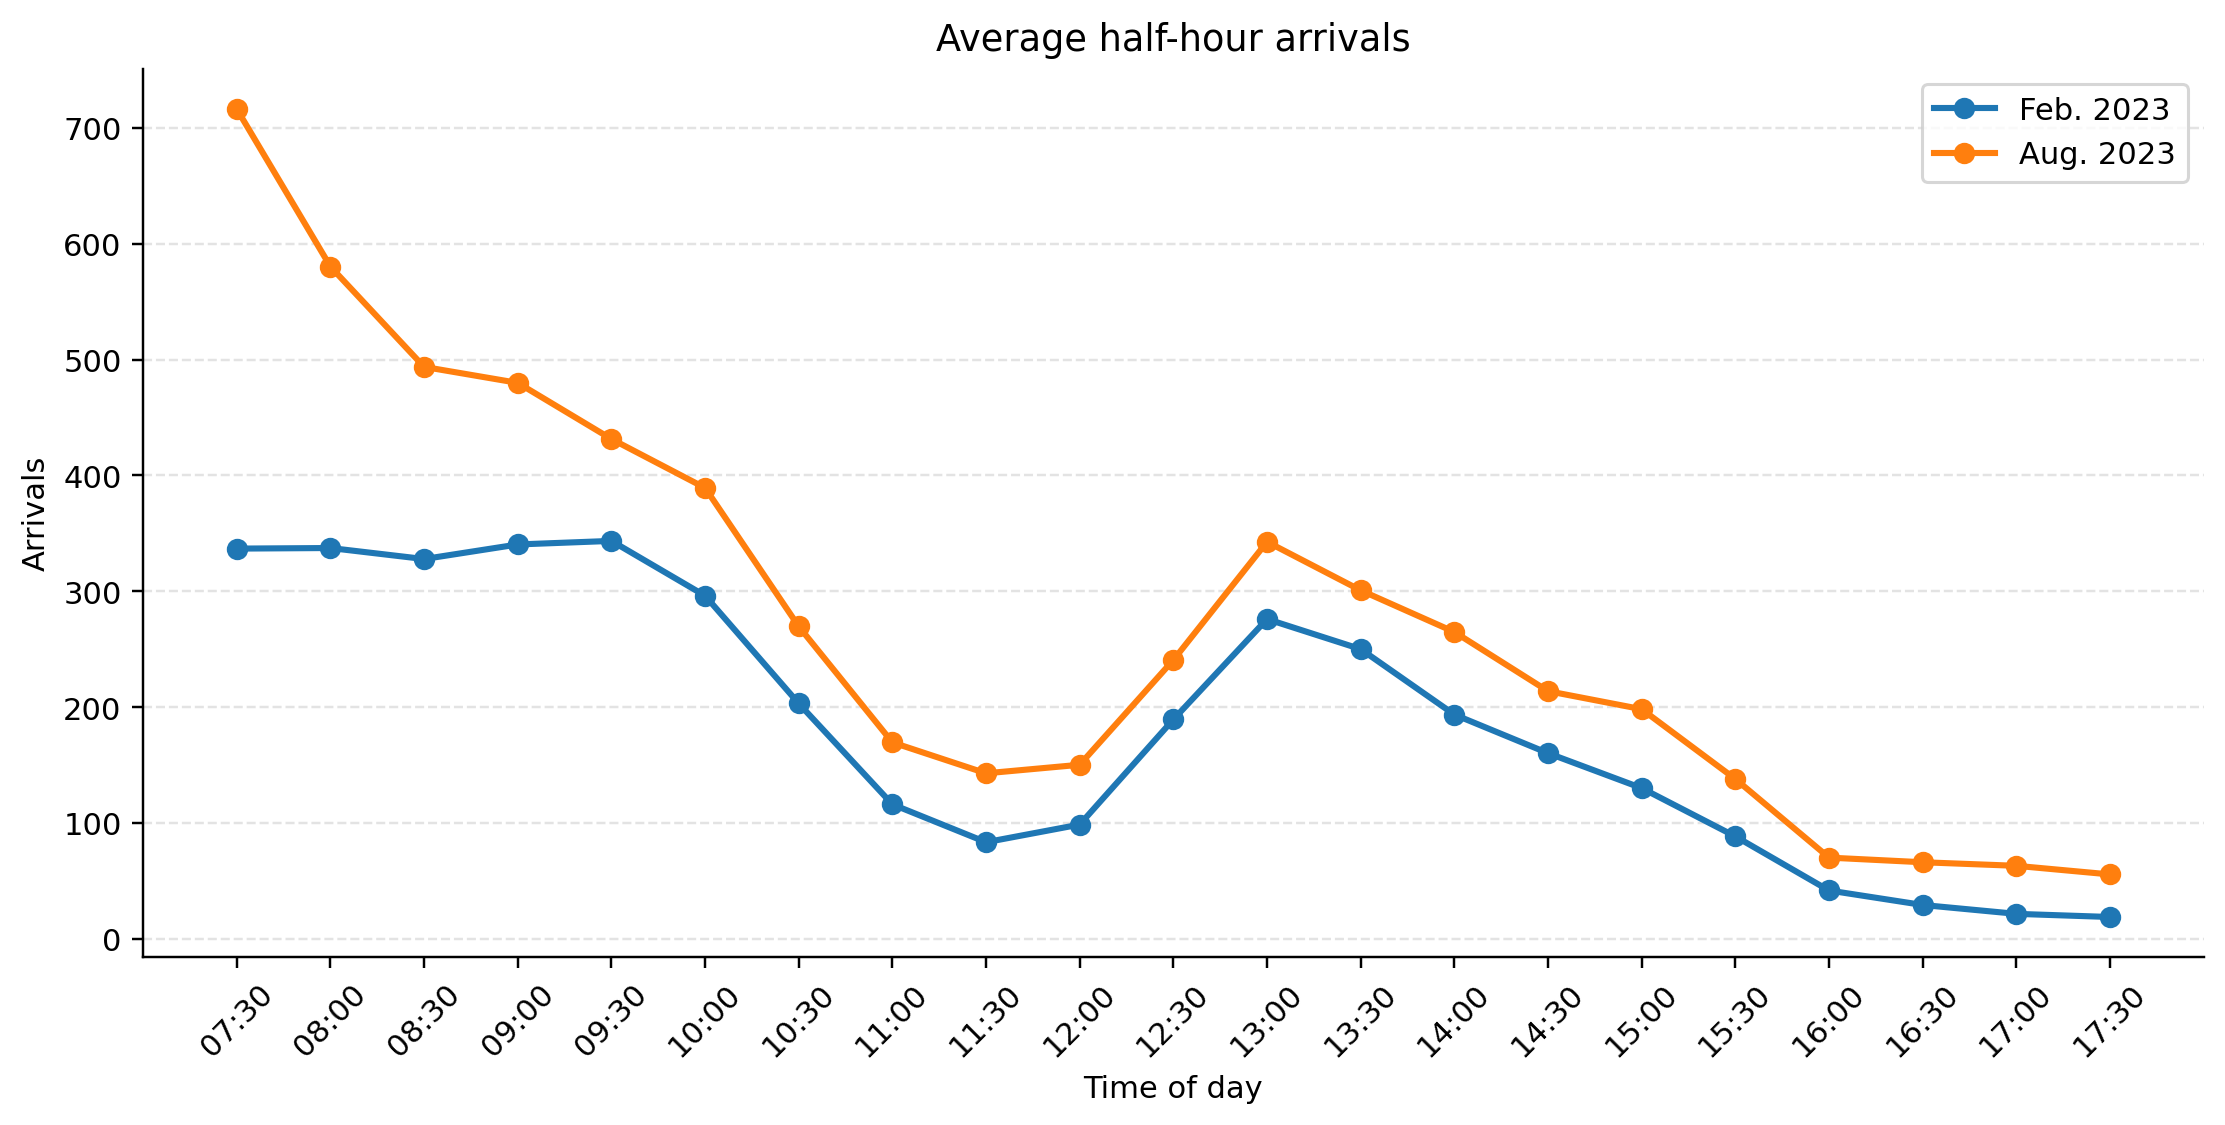
\includegraphics[width=0.86\textwidth]{arrival_profile.png}
  \caption{两期样本的平均半小时到达曲线}
  \label{fig:arrival-profile}
\end{figure}

图\ref{fig:service-distribution}展示了有效问诊时长代理的经验分布。两期样本都呈现明显右偏：大量患者服务时长较短，但仍存在一部分记录对应较长服务过程。这一事实支持Model 2引入随机服务需求。如果只使用平均服务时间，模型可能低估长服务患者在高峰时段对队列尾部风险的放大作用；但由于结束时点为代理变量，该结论仍需在更精确的诊间行为数据中复核。

\begin{figure}[H]
  \centering
  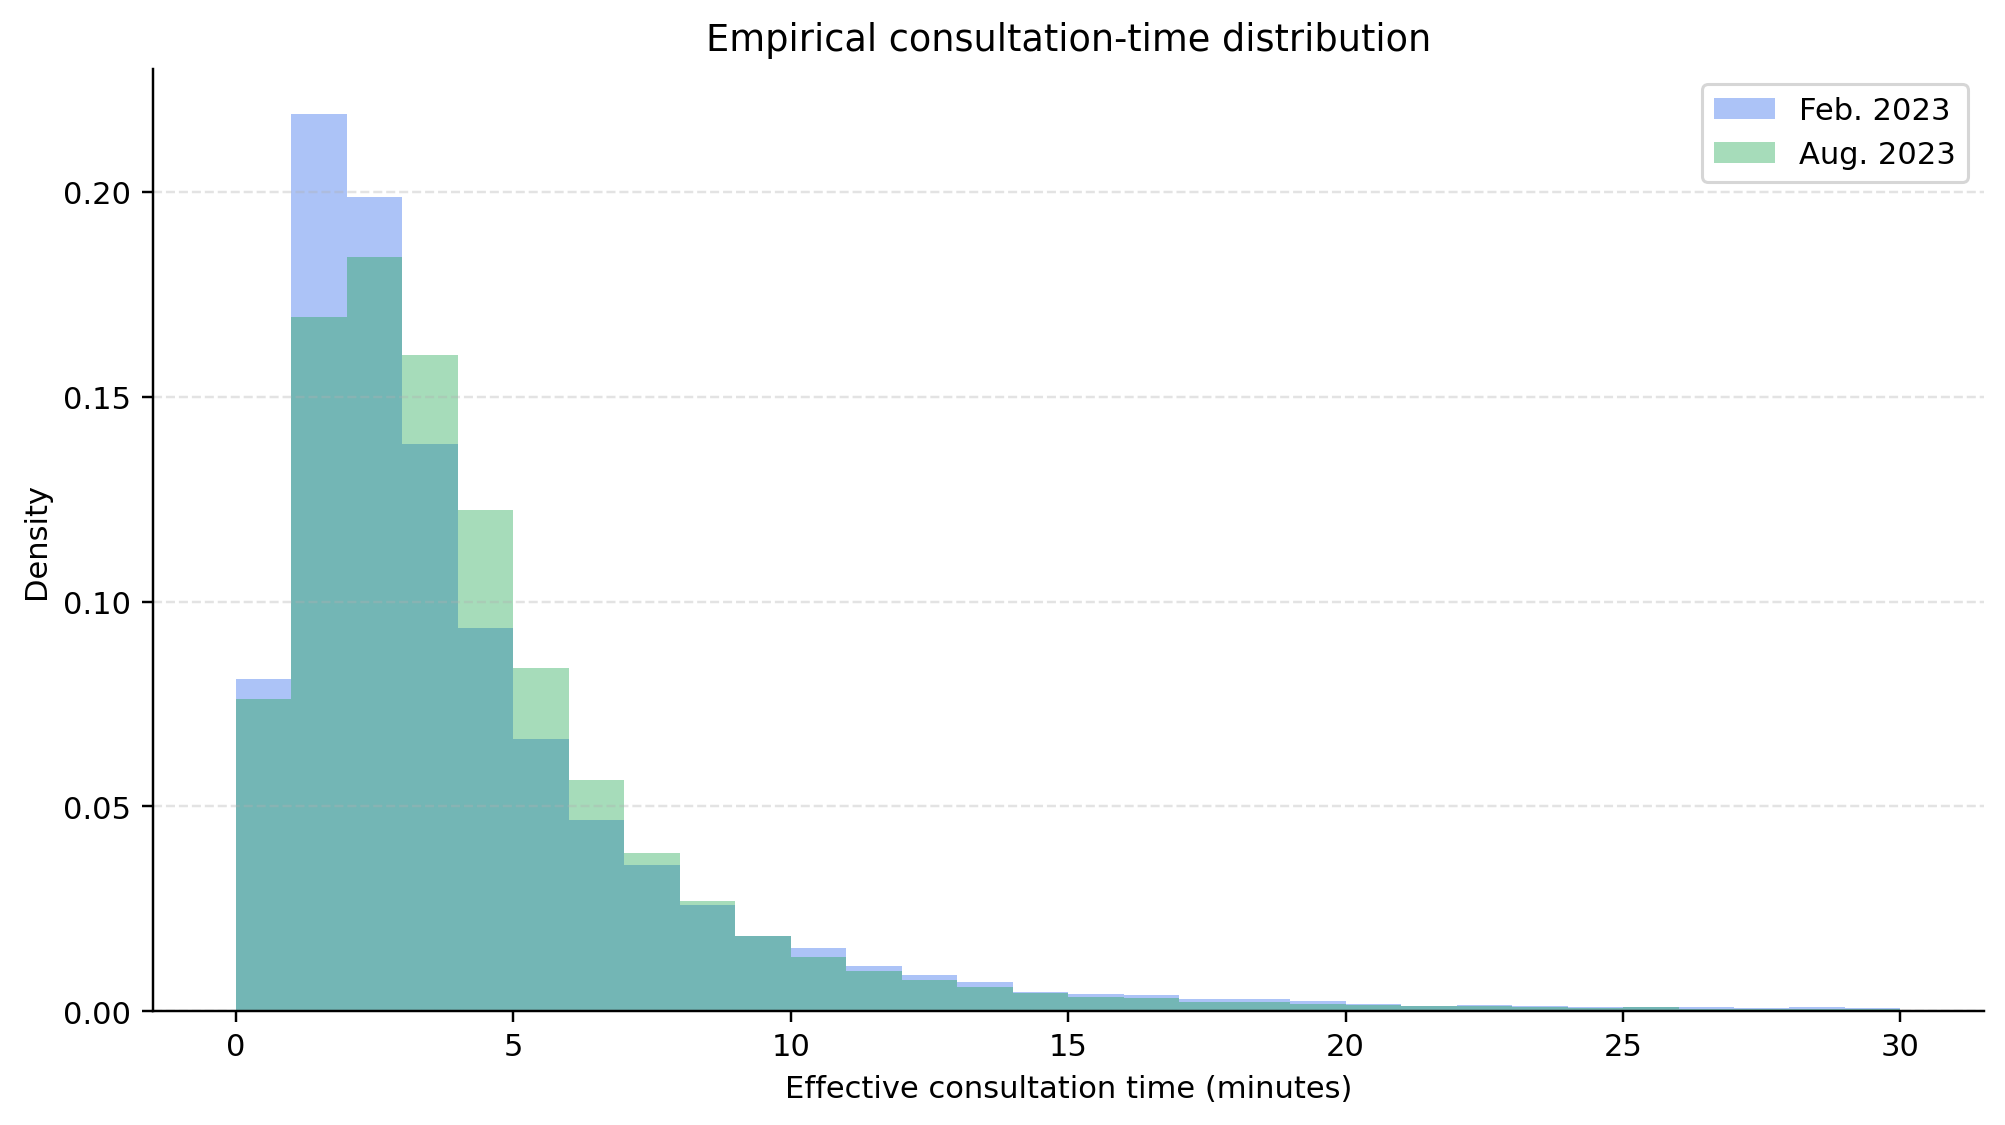
\includegraphics[width=0.82\textwidth]{service_distribution.png}
  \caption{有效问诊时长经验分布（图中展示30分钟以内记录）}
  \label{fig:service-distribution}
\end{figure}

\subsection{模型参数标定}

表\ref{tab:parameter-calibration}给出了主要参数的经验标定结果。固定服务时长参数$s_{\mathrm{base}}$可取样本平均服务时长；随机服务需求不再被压缩为某个特定分布，而是直接使用样本均值、标准差和分位数刻画其一阶、二阶和尾部特征。到达过程使用两类离散系数刻画$\kappa$的经验量级：全院半小时到达离散系数用于描述总体峰值聚集；模型原型在医生-日期-半小时状态上使用医生-时段到达离散系数，并向月度半小时离散系数收缩以降低14天小样本噪声。安全阈值$C_{\mathrm{safe}}$使用医生局部队列与时段到达需求形成的风险负载95\%分位数作为参考，因此它对应单医生或单诊室压力阈值，而不是全院聚合队列阈值，也不是外部给定的临床安全标准。两个样本窗口分别使用各自的$C_{\mathrm{safe}}$，所以跨窗口比较时应关注到达、等待和状态占比的相对模式，而不能把阈值数值本身解释为8月系统更安全或更危险。若医院在实际部署中希望进一步提高精度，应使用更长时间窗、分科室经验分布、负二项到达或离散事件仿真检验近似误差。

\begin{table}[H]
\centering
\small
\caption{模型参数的经验标定结果}
\label{tab:parameter-calibration}
\begin{tabular}{lrr}
\toprule
参数或统计量 & 2023年2月样本 & 2023年8月样本 \\
\midrule
$s_{\mathrm{base}}$（分钟） & 4.61 & 4.62 \\
$\sqrt{v}$（服务时长标准差，分钟） & 5.47 & 4.96 \\
服务时长中位数（分钟） & 3.03 & 3.43 \\
服务时长95\%分位数（分钟） & 12.97 & 11.78 \\
局部 $C_{\mathrm{safe}}$ 代理值（分钟） & 110.54 & 143.09 \\
半小时到达离散系数均值 & 3.78 & 4.27 \\
模型局部 $\kappa$ 均值 & 2.61 & 2.89 \\
早高峰挂号占比 & 47.55\% & 45.28\% \\
高频医生平均服务时长变异系数 & 0.54 & 0.55 \\
\bottomrule
\end{tabular}
\end{table}


从表\ref{tab:parameter-calibration}可以看到，半小时到达离散系数均值在两期样本中分别为3.78和4.27，明显高于泊松分布“方差等于均值”的基准；进入模型原型的局部$\kappa$均值也高于1。这意味着真实到达存在过度离散和峰值聚集，正文模型因而使用$\kappa_t$修正服务需求方差。早高峰挂号占比接近一半，说明门诊风险并非均匀分布在全天，而是高度集中在上午前段。高频医生平均服务时长变异系数约为0.55，说明医生或其服务病例组合之间存在明显差异；由于本文没有完全控制科室、病种和患者类型，该差异只能作为多诊室异质性建模的经验依据，不能简单解释为医生个人能力差异。

\subsection{模型原型的经验标定检验}

在完成参数标定后，本文检验模型原型在医生局部时段层面的可解释性。具体做法是构造“医生-日期-半小时”状态单元，以时段开始待诊人数、该时段新到达人数、医生-时段局部到达离散系数、服务时长均值与方差计算风险调整负载，并将其代入式\eqref{eq:model2-deterministic-rsi}的经验实施形式。由于$\rho$与$\nu$在确定性约束中以乘积形式出现，本文将$\rho\nu$设为经验安全阈值$C_{\mathrm{safe}}$，使方差修正项与队列工作量处于同一量纲。该设定是样本内尺度归一化，不等价于求解理论模型中的最优风险水平$\rho$。

对每个状态，本文不求解完整跨时段动态优化问题，而是求解满足局部风险约束且偏离舒适服务能力最小的目标服务工作量。经验标定中取$c_0=\Delta=30$分钟；服务用时下界取$s_{\min}=\max\{2.0,\hat p_{10}\}$，其中$\hat p_{10}$为医生半小时平均服务用时的10\%分位数；服务能力上界为$c_{\max}=\Delta m/s_{\min}$；赶工惩罚系数取
\begin{equation}
\gamma=\frac{1}{2(c_{\max}-c_0)},\qquad c_{\max}>c_0.
\end{equation}
其中$c_{\max}>c_0$等价于$s_{\min}<m$；若数据边界导致$s_{\min}\geq m$，则应重新设定临床下界或不允许加速。该口径使过度加速在接近上界时产生明显惩罚，但它仍是运营原型设定，不是由临床质量结局估计得到的结构参数。目标服务工作量再由式\eqref{eq:duration-from-capacity}转化为目标平均单人服务用时$s^*$。

\begin{table}[H]
\centering
\small
\caption{模型原型的全窗口内部状态诊断}
\label{tab:model-application}
\begin{tabular}{lrrrrrr}
\toprule
样本窗口 & 状态单元数 & $C_{\mathrm{safe}}$ & 舒适占比 & 调整占比 & 触及下界占比 & $s^*$均值 \\
\midrule
2023年2月 & 18,536 & 100.05 & 98.22\% & 0.95\% & 0.83\% & 4.57 \\
2023年8月 & 28,707 & 133.35 & 97.62\% & 0.93\% & 1.45\% & 4.57 \\
\bottomrule
\end{tabular}
\end{table}


表\ref{tab:model-application}显示，在上述样本内阈值和参数口径下，两期样本中绝大多数状态在舒适节奏下即可满足局部风险约束，说明模型原型不会机械地要求医生持续加速；其作用主要体现在识别少量高压状态并给出服务节奏、支援或分流提醒。2月样本中，需要节奏调整但未触及服务用时下界的状态占0.86\%，触及下界的状态占0.94\%；8月样本对应比例分别为1.01\%和1.42\%。这些比例表明两个窗口中均存在尾部高压状态，但由于$C_{\mathrm{safe}}$按窗口分别标定，不能仅凭该表断言某一月份的模型风险水平更高。触及下界的状态尤其应被解释为需要管理支援或容量调整，而不是要求医生继续压缩问诊时间。

\subsection{模型目标服务用时的反馈策略拟合}

在获得模型目标服务用时$s^*$后，本文再比较式\eqref{eq:feedback-linear}、式\eqref{eq:feedback-exp}和式\eqref{eq:feedback-power}三种参数化反馈策略。此时因变量不再是观测到的实际平均服务用时，而是由模型原型和式\eqref{eq:duration-from-capacity}给出的目标服务用时；解释变量为该半小时开始时医生名下的待诊人数。由于本节以医生为局部状态单元，可近似取$N_{it}=1$，故$q_{it}=Q_{it}$。线性型策略直接用最小二乘估计；指数型策略先对$s^*$取对数后估计；幂函数型策略则对$s^*$和$1+q_t$分别取对数后估计。为保证结果可比，本文将三类策略的预测值均还原到分钟尺度，并在原始分钟尺度上比较$R^2$、RMSE和AIC。估计结果见表\ref{tab:feedback-estimates}。

\begin{table}[H]
\centering
\small
\caption{模型目标服务用时的反馈策略拟合与比较}
\label{tab:feedback-estimates}
\begin{tabular}{llrrrrr}
\toprule
样本窗口 & 策略形式 & $\hat a$ & $\hat b$ & $R^2$ & RMSE & AIC \\
\midrule
2023年2月 & 线性型 & 4.696 & 0.021 & 0.211 & 0.248 & -51704.2 \\
2023年2月 & 指数型 & 4.736 & 0.006 & 0.160 & 0.256 & -50532.7 \\
2023年2月 & 幂函数型 & 4.720 & 0.022 & 0.045 & 0.273 & -48160.3 \\
2023年8月 & 线性型 & 4.749 & 0.021 & 0.282 & 0.287 & -71658.4 \\
2023年8月 & 指数型 & 4.810 & 0.007 & 0.207 & 0.302 & -68807.4 \\
2023年8月 & 幂函数型 & 4.812 & 0.030 & 0.056 & 0.329 & -63801.6 \\
\bottomrule
\end{tabular}
\end{table}


表\ref{tab:feedback-estimates}显示，三类策略均给出负向队列响应：待诊人数越多，模型建议的目标平均单人服务用时越短。线性型策略在2月样本中的估计为$s_t^*=4.696-0.021q_t$，在8月样本中的估计为$s_t^*=4.749-0.021q_t$；指数型策略在两期样本中的衰减系数约为0.006--0.007；幂函数型策略在两期样本中的弹性系数分别为0.022和0.030。若按原始分钟尺度比较，线性型策略在两期样本中均具有更高的$R^2$、更低的RMSE和更低的AIC，指数型策略次之，幂函数型策略相对较弱。需要注意的是，线性型$R^2$分别为0.211和0.282，说明单一队列长度只能解释模型目标用时的一部分变化；三类策略拟合的是模型生成目标服务用时，而不是直接拟合实际问诊行为，更不是在线干预效果。其意义在于把复杂模型输出压缩为便于看板展示的简化规则。图\ref{fig:feedback-policy}展示了三类反馈策略对模型目标服务用时的拟合曲线。

\begin{figure}[H]
  \centering
  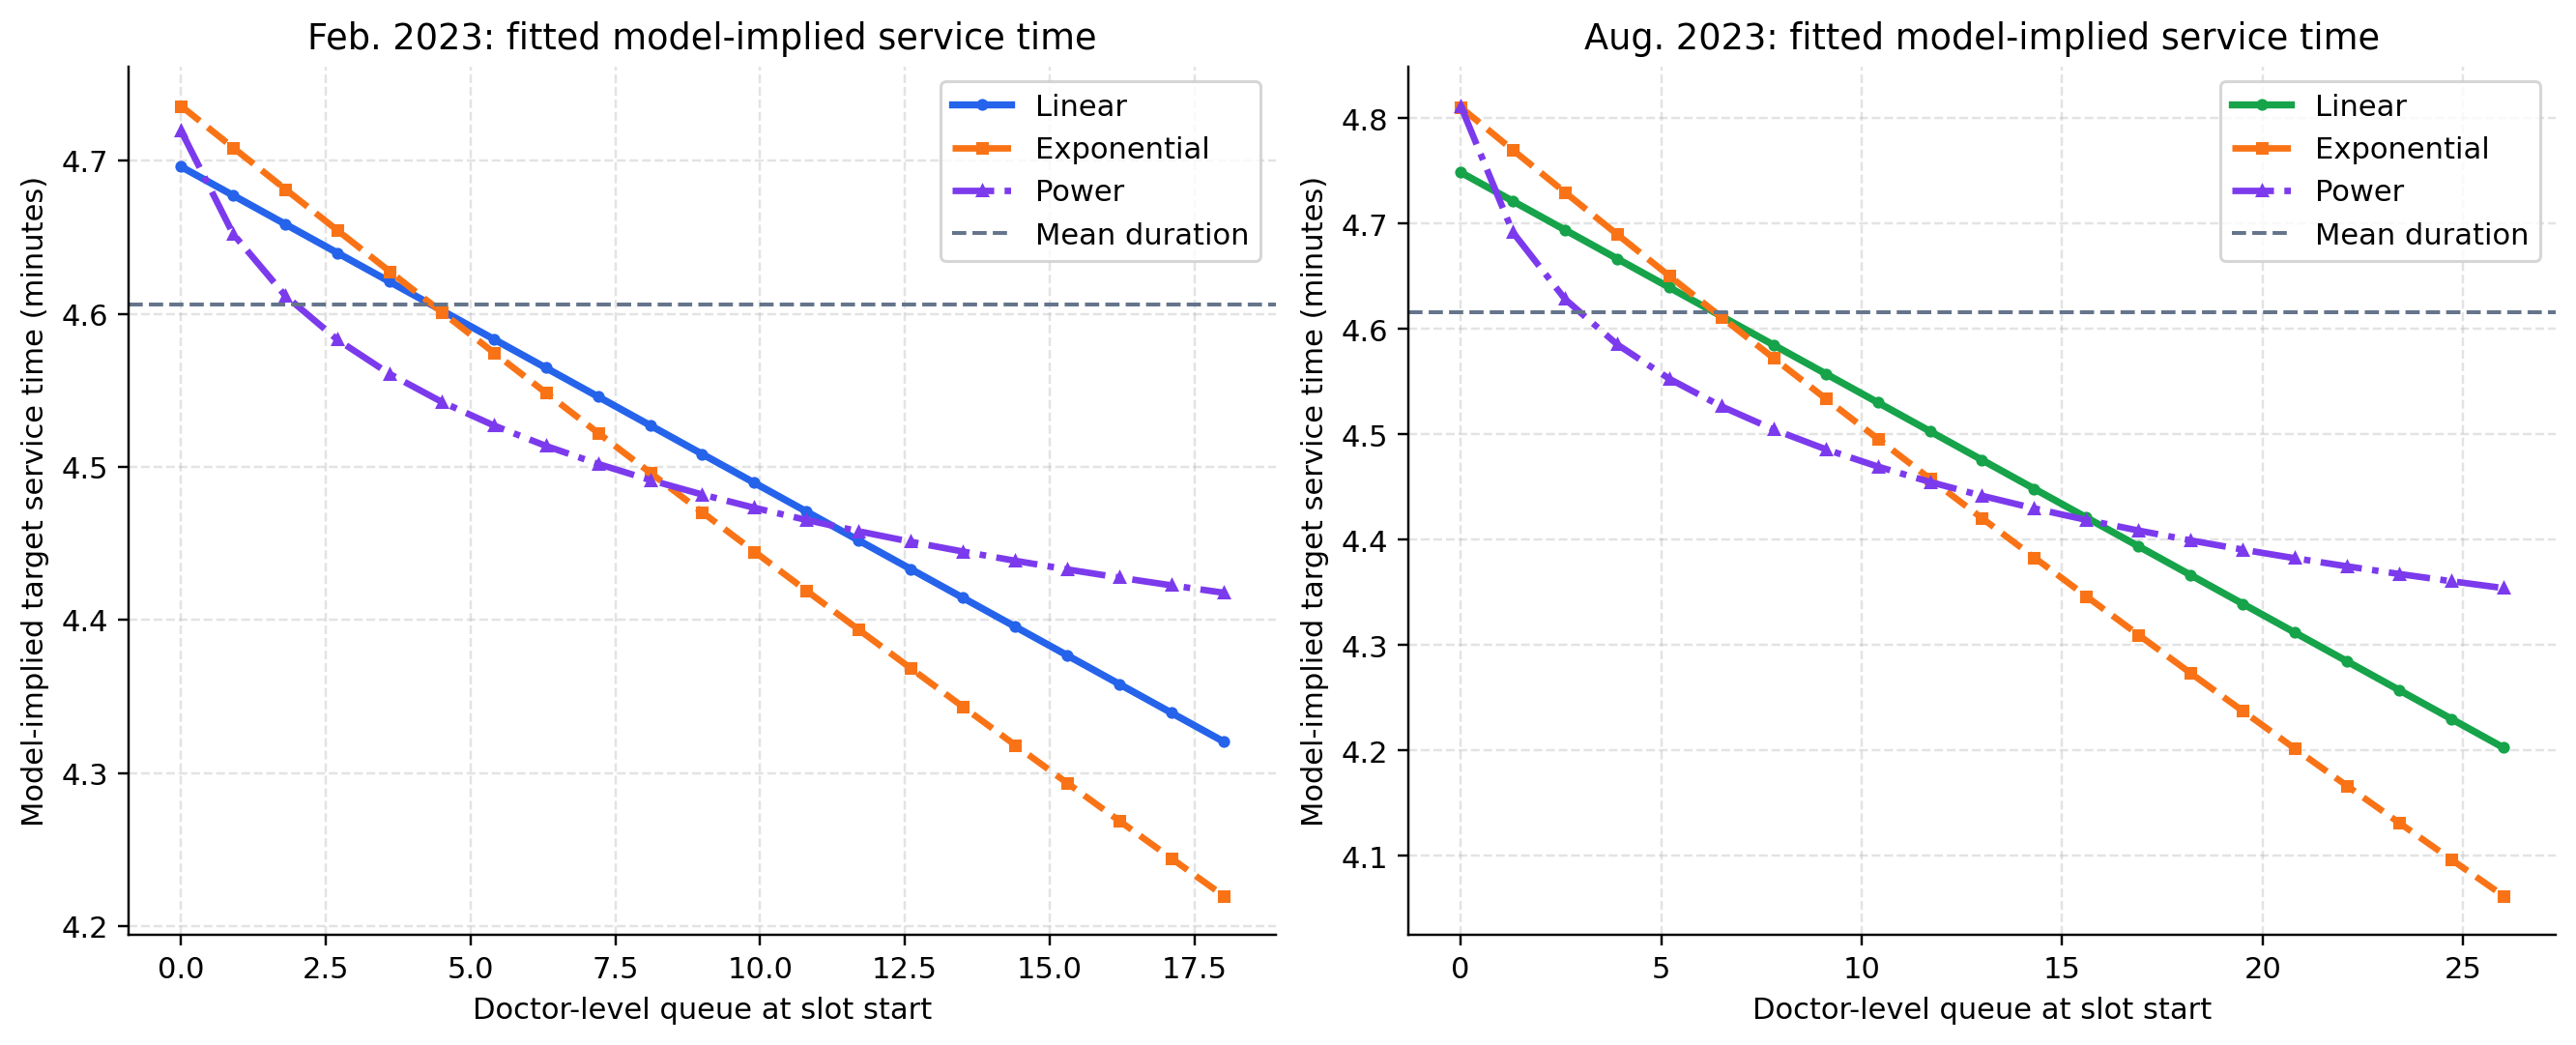
\includegraphics[width=0.9\textwidth]{feedback_policy.png}
  \caption{线性型、指数型与幂函数型反馈策略拟合曲线}
  \label{fig:feedback-policy}
\end{figure}

\section{管理启示与实施建议}

\subsection{从平均效率管理转向尾部风险管理}

实证结果显示，两期样本平均服务时长代理几乎相同，但等待时间和风险负载差异明显。这提示门诊拥堵不能只从平均诊疗速度解释，还需要关注高峰到达、预约负载和诊室异质性共同形成的尾部风险。医院若只跟踪日均挂号量、平均等待和平均利用率，容易低估早高峰拥堵。因此，建议在门诊管理看板中加入半小时到达离散系数、风险负载95\%分位数、高压时段占比和触及服务用时下界的状态数等指标。上述指标应作为预警工具，而非单独作为压缩医生问诊时间的考核依据。

\subsection{将医生赶工成本纳入调度边界}

本文模型强调，服务能力提升并非免费。医生在高峰期适度调整节奏可能降低队列，但如果长期处于高强度赶工状态，可能损害医患沟通和诊疗质量。由于服务用时建议会通过$c_{it}=N_{it}\Delta m_i/s_{it}$转化为服务工作量，医院在实施动态服务用时建议时，应把$s_{\min}$设置为不可突破的安全边界，并将$c_{\max}$作为短时应急上限，而不是常态工作标准。本文实证中的$s_{\min}$来自审慎的数据边界，并非临床质量标准；真实部署前应由科室专家、医疗质量部门和伦理管理共同确定。对于持续高负荷科室，应优先通过预约容量平滑、增开诊室、弹性支援和可行跨诊室分流解决，而不是依赖医生长期加速。

\subsection{用服务用时反馈支持实时但克制的调度}

队列反馈策略的价值在于简单、透明和可解释。医院信息系统可以实时读取候诊人数，使用模型原型计算目标服务用时，再按线性型反馈策略给出近似提示，并依据式\eqref{eq:feedback-capacity}折算为服务工作量，与风险阈值、赶工边界进行校验。当待诊人数较低时，系统不提示加速；当队列超过阈值时，系统优先触发支援、分流、预约平滑或延后非紧急需求等管理动作，服务节奏压缩只应作为短时辅助选项。该机制不要求医生理解复杂优化模型，只需将模型结果嵌入调度看板或分诊系统。指数型和幂函数型可作为敏感性分析工具，用于检查服务用时是否呈现明显的非线性衰减特征。

\section{结论与展望}

\subsection{研究结论}

本文围绕门诊服务能力控制中的排队风险与服务节奏边界问题，构建了基于资源满意度思想的模型原型，并使用真实门诊数据进行了描述性分析、参数标定和样本内策略近似。主要结论如下：

\begin{enumerate}
  \item 门诊拥堵应使用尾部敏感指标刻画。真实数据中半小时到达存在明显过度离散，平均值不能充分反映早高峰风险，因此模型中需要纳入到达离散系数$\kappa_t$。
  \item 服务时长随机性是门诊风险的重要来源。两期样本平均服务时长代理较稳定，但服务分布右偏，长服务患者可能放大高峰期排队压力。
  \item 医生和诊室异质性较为明显。高频医生平均服务时长变异系数约为0.55，为多诊室异构参数设定提供了经验依据，但该异质性可能同时反映科室、病例组合和记录口径差异。
  \item 服务能力决策可以转化为服务用时反馈。通过$c_{it}=N_{it}\Delta m_i/s_{it}$，模型中的服务工作量决策能够映射为医生和管理者可理解的平均单人服务用时建议，但该建议应服从临床判断和安全边界。
  \item 模型原型可用于识别尾部高压状态。在样本内阈值下，两期样本中多数状态在舒适节奏下满足局部风险约束，少量高压状态需要服务节奏调整、支援或触及服务用时下界。触及下界不意味着继续加速，而意味着需要容量或分流干预。
  \item 线性型、指数型和幂函数型队列反馈策略均能近似模型目标服务用时随局部队列压力升高而下降的趋势，其中线性型在两期样本内具有相对更好的原始尺度拟合表现。但其解释力有限，且拟合对象是模型目标而非实际问诊行为。
\end{enumerate}

\subsection{不足与未来研究}

本文仍存在若干不足。第一，两个样本窗口均为14天，能够支持模型标定示例，但不足以识别长期季节规律、星期效应或公共卫生事件冲击。第二，服务结束时点来自代理字段，有效问诊时长可能混入检查、缴费或系统记录延迟，未来应使用更精确的诊间进入和离开时间。第三，本文虽引入到达离散系数修正，但局部$\kappa$仍来自短窗口收缩估计，确定性约束也仍依赖正态近似，未来应使用负二项到达、经验服务分布或离散事件仿真进行稳健性验证。第四，二次凸赶工惩罚是运营代理，尚未由患者安全、复诊、投诉、满意度或医生疲劳等质量结果标定。第五，经验部分将$\rho\nu$设为样本内安全阈值以完成尺度归一化，这不等价于估计理论风险偏好参数。第六，服务用时反馈策略由同一样本估计，尚未进行样本外预测、滚动优化、基准策略对照或真实在线干预验证。未来研究可结合医院信息系统开展滚动仿真或小范围试点，同时比较固定服务节奏、预约容量平滑、弹性支援和队列反馈等策略对等待时间、医生负荷和患者体验的综合影响。

\section*{代码与复现说明}
\addcontentsline{toc}{section}{代码与复现说明}

本文数据清洗、参数标定、表格生成和绘图代码位于\path{src/posts/Business Paper/Graduate/}目录。运行\path{analyze_data.py}可由\path{data.ods}生成\path{analysis_results.json}和\path{analysis_results.md}；运行\path{make_figures.py}可生成本文使用的\path{figures/*.png}和\path{tables/*.tex}。所有论文图片均由matplotlib生成，论文主文件通过\verb|\input{tables/...}|和\verb|\includegraphics{figures/...}|引用输出结果。

\newpage
\bibliographystyle{plainnat}
\bibliography{references}

\end{document}
